\section{问题四建模与求解}

为分析不同类别的玻璃样本的化学成分的关联关系,并比较它们之间关联关系的差异性,利用灰色关联性分析模型并比较它们之间的差异性,做出流程图如下:

\begin{figure}[H] 
	\centering %图片居中
	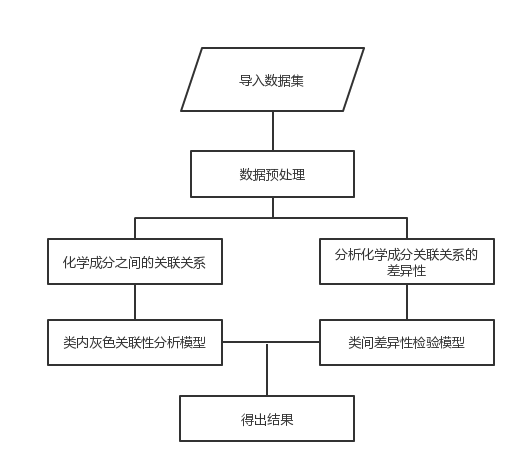
\includegraphics[width=0.7\textwidth]{22.png} %插入图片,[]中设置图片大小,{}中是图片文件名
	\caption{问题四流程图} %最终文档中希望显示的图片标题
	\label{Fig.main23} %用于文内引用的标签
\end{figure}


\subsection{数据预处理}

上述问题中处理后(补齐缺失值,删减异常值)的高钾玻璃数据表和铅钡玻璃数据表来进行类内的关联性分析,另外进行类间相关性分析。

\subsection{类内灰色关联性分析模型}

\subsubsection{模型准备}

对于类内各数据之间的关系,常见思路是进行相关系数矩求解,而求解相关性矩阵要进行正态性检验,本问对高钾玻璃和铅钡玻璃分别进行正态性检验,经过检验发现大部分特征都不满足正态分布(具体数据见附件)。因此,本问决定采用灰色关联预测进行关联性分析。

\subsubsection{模型建立}

对于灰色关联分析来分析类内的关联性,考虑到类内中每个化学成分之间都可能有关联性,因此用14个特征中随机抽取一个特征与其他特征进行灰色关联性分析。即有:

1. 将数据进行预处理:

\begin{equation}
    \widetilde{{{e}_{kj}}}=\frac{{{e}_{kj}}}{\overline{{{e}_{j}}}},\overline{{{e}_{j}}}=\frac{1}{{{n}_{z}}}\sum\limits_{k=1}^{n}{{{e}_{kj}}}(k=1,2,\cdots ,{{n}_{z}})
\end{equation}

\begin{equation}
    \widetilde{{{f}_{k}}}=\frac{{{f}_{k}}}{\overline{{{f}_{j}}}},\overline{{{f}_{j}}}=\frac{1}{{{n}_{z}}}\sum\limits_{k=1}^{n}{{{f}_{k}}}.
\end{equation}

2. 确定母序列和子序列:

\begin{equation}
    E={{\left[ {{e}_{1}},{{e}_{2}},\cdots ,{{e}_{13}} \right]}^{T}}.
\end{equation}

\begin{equation}
    F=\left[ \begin{matrix}
		{{f}_{11}} & {{f}_{12}} & \cdots  & {{f}_{1,13}}  \\
		{{f}_{21}} & {{f}_{22}} & \cdots  & {{f}_{2,13}}  \\
		\vdots  & \vdots  & \ddots  & \vdots   \\
		{{f}_{{{n}_{z}}1}} & {{f}_{{{n}_{z}}2}} & \cdots  & {{f}_{{{n}_{z}}13}}  \\
	\end{matrix} \right]
\end{equation}

3. 计算序列和母序列的关联系数:


\begin{equation}
    r=\underset{j}{\mathop{\min }}\,\underset{k}{\mathop{\min }}\,|{{f}_{0}}(k)-{{f}_{j}}(k)|
\end{equation}

\begin{equation}
    b=\underset{j}{\mathop{\max }}\,\underset{k}{\mathop{\max }}\,|{{f}_{0}}(k)-{{x}_{j}}(k)|
\end{equation}

4. 计算关联度:

(1)构造:

\begin{equation}
    {{a}_{k,q}}={{\xi }_{q}}(k)=\frac{r+\rho b}{|{{e}_{kq}}-{{f}_{q}}|+\rho b}.
\end{equation}

(2)计算关联度:

\begin{equation}
    R=\frac{1}{{{n}_{z}}}\sum\limits_{k=1}^{n}{{{\xi }_{q}}(k)}=\frac{1}{{{n}_{z}}}\sum\limits_{k=1}^{n}{{{a}_{kq}}}.
\end{equation}

\subsubsection{模型求解}

根据公式可以分别算出高钾与铅钡的类内的灰色关联结果(下表为高钾玻璃灰色关联结果,铅钡结果见附件)

\begin{figure}[H] 
	\centering %图片居中
	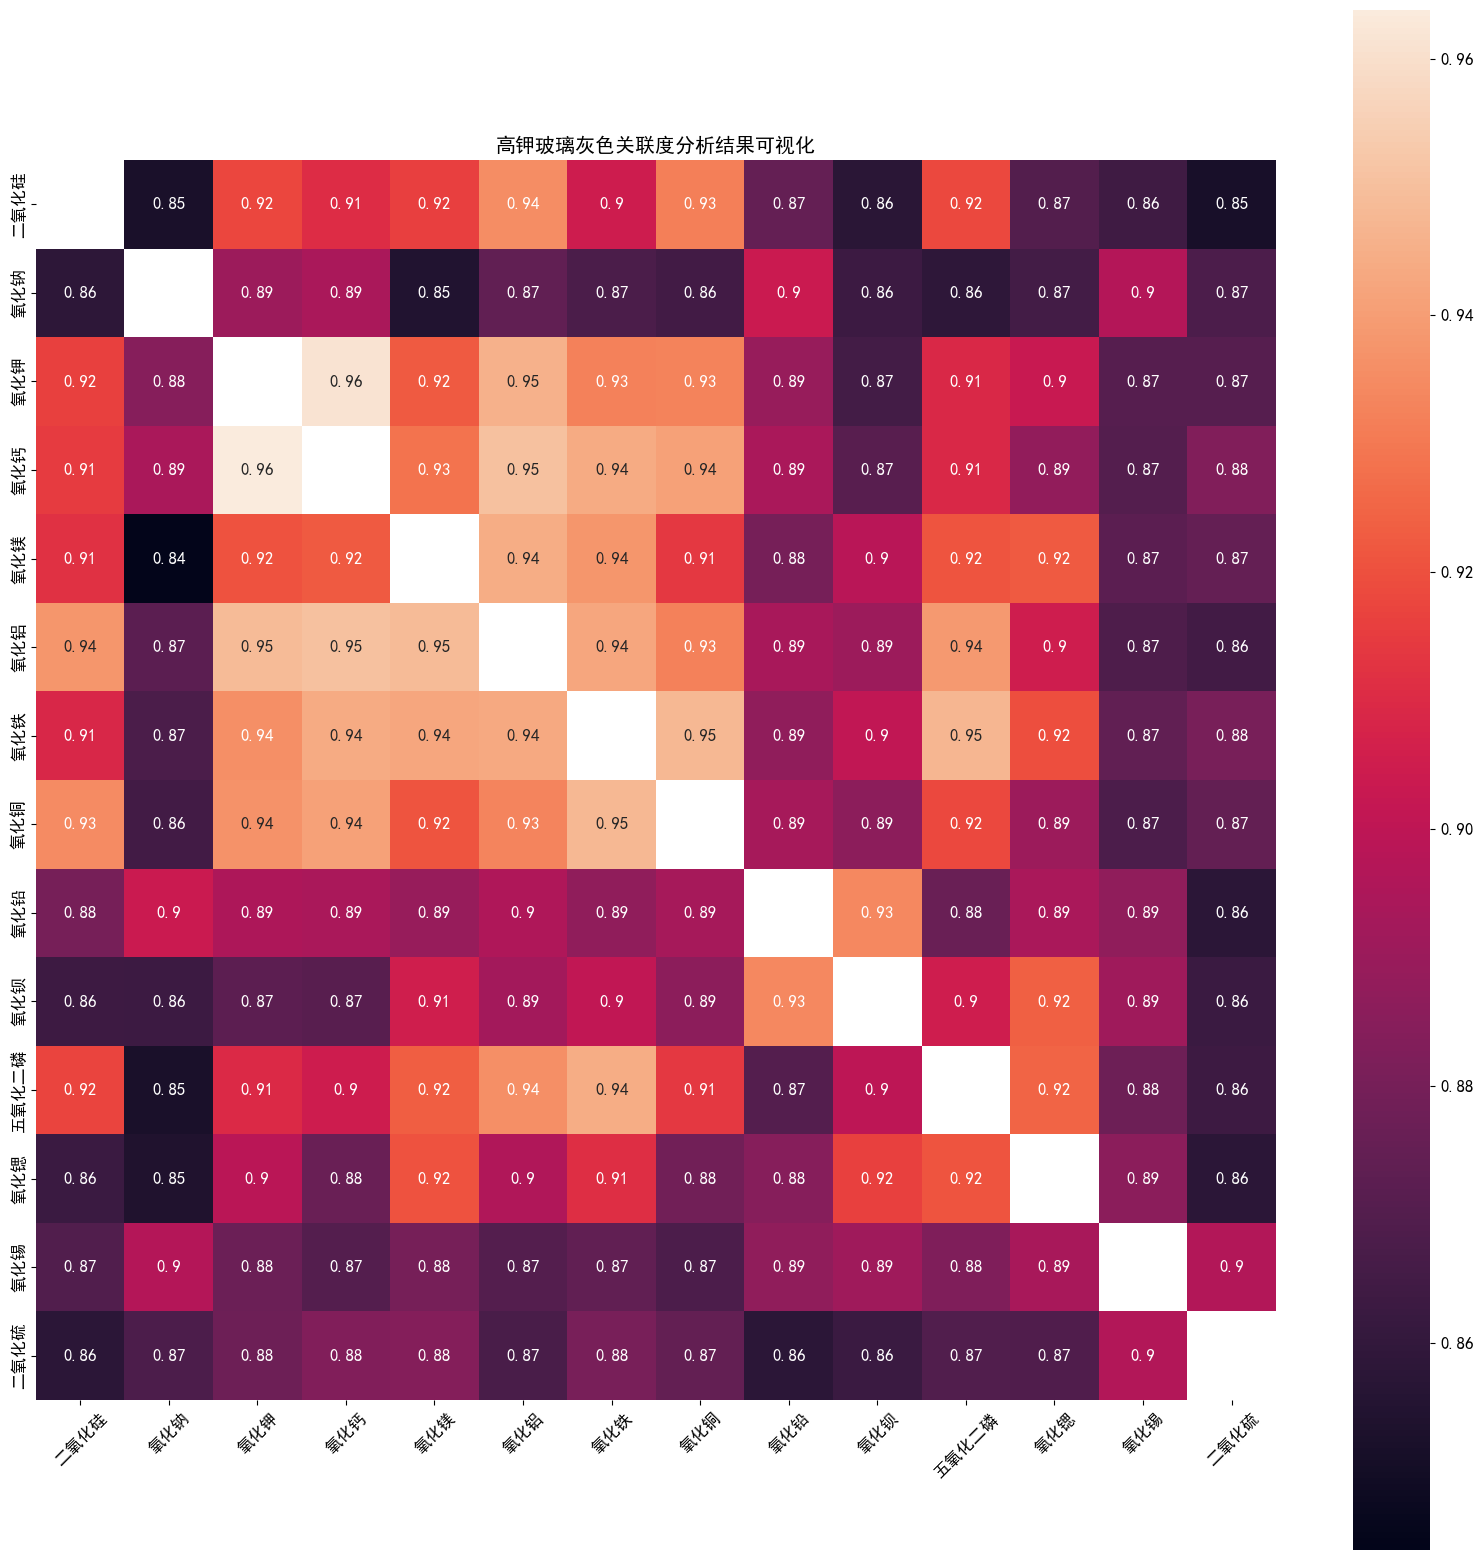
\includegraphics[width=0.7\textwidth]{23.png} %插入图片,[]中设置图片大小,{}中是图片文件名
	\caption{高钾玻璃关联度分析结果可视化图} %最终文档中希望显示的图片标题
	\label{Fig.main24} %用于文内引用的标签
\end{figure}

由图20可以看到每个化学成分之间的关联度结果最低为0.84,即整个类内的化学物质之间都存在的显著关联性,可以判断出在同类化学成分之间每种成分之间都存在关联关系。


\subsection{类间差异性检验模型}

\subsubsection{模型建立}

本问基于类内灰色关联得到的高钾类各化学成分与铅钡类化学成分的关联系数组成新的关联的系数表,需要对类间的同一化学成分关联性的差异性进行分析,配对t检验是一种用于配对定量数据之间的差异对比关系的优良检验方法。首先需要对两类数据进行正态性检验,检验之后发现都不满足正态分布。需要使用其他检验方法,因此使用非参数检验,本问所求两种类型同一化学成分的差异性可以采用非参数配对样本Wilcoxon符号秩检验进行检验。

\subsubsection{模型求解}

利用spasspro中的非参数检验配对样本Wilcoxon符号秩检验对于新表数据进行差异性检验,得出两类玻璃的同一化学物质的差异性显著系数表。

\begin{table}[H]
	\centering
	\begin{tabular}{c c c} 
		\toprule[1.5pt]
		化学成分 & 值(显著性) & Cohen's d值(差异幅度) \\
		\midrule[1pt]
		二氧化硅 & 0.116 & 0.427 \\
		氧化钠 & 0.221 & 0.23 \\
		氧化钾 & 0.101 & 0.373 \\
		氧化钙 & 0.600 & 0.139 \\
		氧化镁 & 0.507 & 0.088 \\
		氧化铝 & 0.753 & 0.013 \\
		氧化铁 & 0.087* & 0.359 \\
		氧化铜 & 0.807 & 0.059 \\
		氧化铅 & 0.013** & 0.727 \\
		氧化钡	& 0.016** &	0.625 \\
		五氧化二磷 & 0.507 & 0.033 \\
		氧化锶 & 0.064* & 0.453 \\
		氧化锡 & 0.116 & 0.209 \\
		二氧化硫 & 0.002*** & 0.56 \\
		\toprule[1.5pt]
\end{tabular}
\caption{差异性显著系数表}
\end{table}

由$p>0.05$可以判定上表两种类间化学成分中二氧化硅、氧化钠、氧化钾、氧化钙、氧化镁、氧化铝、氧化铁、氧化铜、五氧化二磷、氧化锶、氧化锡不能拒绝显著性假设,故两个量之间不存在显著性差异。

由$p\leq 0.5$可以判定上表两种类间化学成分中氧化铅、氧化钡、二氧化硫能拒绝显著性假设,故两个量之间存在显著性差异。

当两个变量之间具有显著性差异时,Cohen's d值一般都较大,说明两个变量之间有较大的差异幅度。
